\documentclass{beamer}

\usepackage[utf8]{inputenc}

\usepackage{fancyvrb}
\usepackage{hyperref}
\usepackage{tikz}
\usepackage{xcolor}

\usetikzlibrary{arrows, positioning}

\title[git]{git --- an introduction}
\subtitle{Learning to commit}
\author{LiTHe kod}
\date{2021}

\logo{\vspace{-5.0em}
\includegraphics[width=.06\textwidth]{watermark.png}\hspace*{.93\paperwidth}}

\newcommand{\temporalgray}[2]{\temporal<#1>{\phantom{#2}}{#2}{\textcolor{gray}{#2}}}
\newcommand{\keyword}[1]{\hspace{-1.0em}\colorbox{black}{\textcolor{white}{\textbf{#1}\vphantom{Ep}}}\vspace{0.2em}} % yikes
\newcommand{\command}[1]{\texttt{\textcolor{gray}{\$} {#1}}}

\begin{document}

\frame{\titlepage}
\frame{\tableofcontents}

%TODO about us

\begin{frame}[fragile]
  \frametitle{LiTHe kod? Tell me more!}
  Your one stop shop for Game Jams, competitive programming, meetups and other coding related events.

  \vspace{2.0em}
  Applications are open for the 21/22 board! \\
  Mail any questions to \texttt{ordf@lithekod.se} \\
\end{frame}

\section{Getting started}

\begin{frame}[fragile]
  \begin{center}
    \Huge \colorbox{black}{\textcolor{white}{DON'T}} \\
    \Huge \colorbox{black}{\textcolor{white}{PANIC}}
  \end{center}
\end{frame}

\begin{frame}[fragile]
  \frametitle{What even is git?}

  Version control that doesn't care about your feelings. \\

  \vspace{1em}
  \keyword{Pros}
  \begin{itemize}
    \item Works offline
    \item Fast
    \item Easy to pronounce
    \item Very powerful
  \end{itemize}

\end{frame}

\begin{frame}[fragile]
  \frametitle{What even is git? \dots and why is it better than email?}

  Why emaijl/Droipbox/whatever isn't the best \\
  version control system -- unlike git.\\
  \vspace{1em}
  \keyword{Cons}
  \begin{itemize}[<+->]
    \item Hard to spell \& pronounce -- unlike git
    \item Hard to see what has changed -- unlike git
    \item Requires constant internet -- unlike git
    \item Cannot do automatic merges  -- unlike git
    \item Slow -- unlike git
  \end{itemize}
  \vspace{1em}
  
  So what are \emph{you} waiting for!
\end{frame}

\begin{frame}[fragile]
  \frametitle{Getting started -- Getting binaries}
  
  Windows: git BASH, \url{gitforwindows.org} or via WSL\\
  macOS: homebrew, \url{git-scm.com}\\
  Linux: Probably already installed\\

\end{frame}

\begin{frame}[fragile]
  \frametitle{Getting started -- Telling git who you are}

  Your name:\\
  \command{git config --global user.name "kodapan"} \\[1em]

  Your email:\\
  \command{git config --global user.email "kodapan@lithekod.se"} \\

\end{frame}

\begin{frame}[fragile]
  \frametitle{Getting started -- Getting your repository}
  \begin{tabular}{ll}
    \command{git clone} & \\
    \command{git init} & \\
  \end{tabular}
\end{frame}

\AtBeginSection[] % Do nothing for \section*
{
\begin{frame}<beamer>
\frametitle{Outline}
\tableofcontents[currentsection]
\end{frame}
}

\section{Basic commands}
\subsection{Getting to know the family}

% Edvard
\begin{frame}[fragile]
  \frametitle{Getting to know the family}

  \begin{tabular}{ll}
    \command{git add} & I want to keep these! \\
    \command{git commit} & I did a thing! \\
    \command{git push} & I want to share this! \\ % mention pull
  \end{tabular}
  \\ [2.0em]

  \texttt{add}, \texttt{commit}, \texttt{push} and \texttt{pull}\textsuperscript{*}
  are the four horsemen of version control. The bread and butter.
  \\ [2.0em]

  \small \textsuperscript{*}\texttt{pull} will be discussed later.

  \vspace{2em}

  \tikzset{->,        % edges are arrows
           >=stealth  % arrow heads are bold
  }

  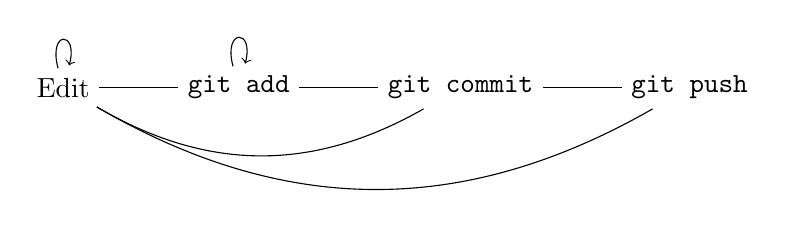
\begin{tikzpicture}
    \node (edit) {Edit};
    \node (add) [right=of edit] {\texttt{git add}};
    \node (commit) [right=of add] {\texttt{git commit}};
    \node (push) [right=of commit] {\texttt{git push}};

    \draw (edit) edge (add);
    \draw (add) edge (commit);
    \draw (commit) edge (push);

    \draw (edit) edge[loop above] (edit);
    \draw (add) edge[loop above] (add);

    \draw (commit) edge[bend left, below] (edit);
    \draw (push) edge[bend left, below] (edit);
  \end{tikzpicture}

\end{frame}

\begin{frame}
  \frametitle{Getting to know the family -- add}
  \keyword{When}\\
    You have made changes that you want to commit.
    Usually the first command in a series of commands.
  \vspace{0.5em}

  \keyword{How}\\
  \hspace{-0.95em}
  \begin{tabular}{ll}
    \command{git add hello.txt} & Stage the specified file \\
    \command{git add *.py} & Stage all python-files \\
  \end{tabular}
  \vspace{0.5em}

  \keyword{Expect}\\
  Silence.
\end{frame}

\begin{frame}[fragile]
  \frametitle{Getting to know the family -- commit}
  \keyword{When}\\
    You have added a \emph{cohesive} group of changes. Making
    the code ready for a new change. Preferably as small as possible.
  \vspace{0.5em}

  \keyword{How}\\
  \hspace{-0.95em}
  \begin{tabular}{ll}
    \command{git commit} & Commit the added file(s) \\
    \command{git commit --amend} & Update the previous commit \\
    \command{git commit -m "msg"} & Specify a message, skips the editor \\
  \end{tabular}
  \vspace{0.5em}

  \keyword{Expect}\\
  A text editor pops up, where you write a descriptive commit message. You will get
  output similar to: \\
\begin{verbatim}
[master 3b65386] A descriptive message
1 file changed, 1 insertion(+)
\end{verbatim}

\end{frame}

\begin{frame}[fragile]
  \frametitle{Getting to know the family -- push}
  \keyword{When}\\
    After you've made commits you are happy with, or if the computer
    is about to blow up. If you haven't pushed, no one knows what
    you've changed. \\
  \vspace{0.5em}

  \keyword{How}\\
  \hspace{-0.95em}
  \begin{tabular}{ll}
    \command{git push} & Tell the server about your changes \\
  \end{tabular}
  \vspace{0.5em}

  \keyword{Expect}\\ [0.1em]
\begin{verbatim}
Enumerating objects: 1, done.
Counting objects: 100% (1/1), done.
Writing objects: 100% (1/1), 192 bytes | 192.00 KiB/s,
  done.
Total 1 (delta 0), reused 0 (delta 0), pack-reused 0
To github.com:kodapan/verkligt.git
   192c869..2ab0e3c  main -> main
\end{verbatim}
\end{frame}

\subsection{Commands for information}

% Gustav
\begin{frame}[fragile]
  \frametitle{Commands for information}

  \begin{tabular}{ll}
    \command{git status} & What is happening? \\
    \command{git diff} & What has changed? \\
    \command{git log} & What has happened? \\
    \command{git show} & What changed over there? \\
  \end{tabular}

\end{frame}

\begin{frame}
  \frametitle{Commands for information -- status}

  \keyword{When}\\
  Always! Guaranteed to not break anything.
  \vspace{0.5em}

  \keyword{How}\\
  \command{git status}
  \vspace{0.5em}

  \keyword{Expect}\\
  Some text explaining what's currently happening.
\end{frame}

\begin{frame}[fragile]
  \frametitle{Commands for information -- status}

\begin{verbatim}
$ git status
\end{verbatim}
\pause{}
\begin{verbatim}
On branch master
nothing to commit, working tree clean
\end{verbatim}
\end{frame}

\begin{frame}[fragile]
  \frametitle{Commands for information -- status}

\begin{verbatim}
$ vim my_file.py
$ git status
\end{verbatim}
\pause{}
\vspace{-3.5ex}
\begin{verbatim}
On branch master
\end{verbatim}
\pause{}
\vspace{-3.5ex}
\begin{verbatim}
Changes not staged for commit:
\end{verbatim}
\pause{}
\vspace{-3.5ex}
\begin{verbatim}
  (use "git add <file>..." to update what will be
   commited)
\end{verbatim}
\pause{}
\vspace{-3.5ex}
\begin{verbatim}
  (use "git checkout -- <file>..." to discard changes
   in working directory)
\end{verbatim}
\pause{}
\vspace{-3.5ex}
\begin{verbatim}

        modified:   my_file.py
\end{verbatim}
\pause{}
\vspace{-3.5ex}
\begin{verbatim}

no changes added to commit (use "git add" and/or
                            "git commit -a")
\end{verbatim}
\end{frame}

\begin{frame}
  \frametitle{Commands for information -- diff}

  \keyword{When}\\
  You want to see the difference between two things. Very versatile.
  \vspace{0.5em}

  \keyword{How}\\
  \command{git diff}
  \vspace{0.5em}

  \keyword{Expect}\\
  A so called \emph{diff}.
\end{frame}

\begin{frame}[fragile]
  \frametitle{Commands for information -- diff}

\begin{verbatim}
$ git diff
\end{verbatim}
\pause{}
\vspace{-2.4ex}
{
\color{gray}
\begin{Verbatim}[commandchars=\\\{\}]
diff --git a/my_file.py b/my_file.py
index a40ce22..ea7235e 100644
--- a/my_file.py
+++ b/my_file.py
\end{Verbatim}
}
\pause{}
\begin{Verbatim}[commandchars=\\\{\}]
@@ -1,5 +1,5 @@
 def main():
\textcolor{red}{-    print("Hello World")}
\textcolor{blue}{+    print("Hello World!")}
 
 if __name__ == "__main__":
     main()
\end{Verbatim}
\end{frame}

\begin{frame}
  \frametitle{Commands for information -- log}

  \keyword{When}\\
  You want to see an overview of what's changed over time.
  \vspace{0.5em}

  \keyword{How}\\
  \command{git log}

  \command{git log <branch>}
  \vspace{0.5em}

  \keyword{Expect}\\
  The log.
\end{frame}

\begin{frame}[fragile]
  \frametitle{Commands for information -- log}
\begin{Verbatim}
$ git add my_file.py
$ git commit
$ git log
\end{Verbatim}
\pause{}
\vspace{-1.2ex} % this spacing can heck off
\begin{Verbatim}
commit 4582c8c2c41d6c7c46bab45d1aae807afacc357e
Author: Kodapan <kodapan@lithekod.se>
Date:   Fri Jan 22 17:48:27 2021 +0100

    add proper punctutation

commit 8e94d9e8bb33496484c80eaff68541dc0b8cccbc
Author: Kodapan <kodapan@lithekod.se>
Date:   Fri Jan 22 17:43:14 2021 +0100

    my first commit
\end{Verbatim}
\end{frame}

\begin{frame}[fragile]
  \frametitle{Commands for information -- log \texttt{--}graph}
\begin{Verbatim}[commandchars=\\\{\}]


$ git log --graph
* commit 4582c8c2c41d6c7c46bab45d1aae807afacc357e
| Author: Kodapan <kodapan@lithekod.se>
| Date:   Fri Jan 22 17:48:27 2021 +0100
| 
|     add proper punctuation
| 
* commit 8e94d9e8bb33496484c80eaff68541dc0b8cccbc
  Author: Kodapan <kodapan@lithekod.se>
  Date:   Fri Jan 22 17:43:14 2021 +0100
  
      my first commit
\end{Verbatim}
\end{frame}

\begin{frame}
  \frametitle{Commands for information -- show}

  \keyword{When}\\
  You want more information about a specific commit.
  \vspace{0.5em}

  \keyword{How}\\
  \command{git show <commit>}
  \vspace{0.5em}

  \keyword{Expect}\\
  Log message and diff output for the commit.
\end{frame}

\begin{frame}[fragile]
  \frametitle{Commands for information -- show}
\begin{Verbatim}[commandchars=\\\{\}]


$ git log --graph
* commit 4582c8c2c41d6c7c46bab45d1aae807afacc357e
| Author: Kodapan <kodapan@lithekod.se>
| Date:   Fri Jan 22 17:48:27 2021 +0100
| 
|     add proper punctuation
| 
* commit 8e94d9e8bb33496484c80eaff68541dc0b8cccbc
  Author: Kodapan <kodapan@lithekod.se>
  Date:   Fri Jan 22 17:43:14 2021 +0100
  
      my first commit
\end{Verbatim}
\end{frame}

\begin{frame}[fragile]
  \frametitle{Commands for information -- show}
\begin{Verbatim}[commandchars=\\\{\}]


$ git log --graph
* commit \textcolor{red}{4582}c8c2c41d6c7c46bab45d1aae807afacc357e
| Author: Kodapan <kodapan@lithekod.se>
| Date:   Fri Jan 22 17:48:27 2021 +0100
| 
|     add proper punctuation
| 
* commit 8e94d9e8bb33496484c80eaff68541dc0b8cccbc
  Author: Kodapan <kodapan@lithekod.se>
  Date:   Fri Jan 22 17:43:14 2021 +0100
  
      my first commit
\end{Verbatim}
\end{frame}

\begin{frame}[fragile]
  \frametitle{Commands for information -- show}
\begin{Verbatim}[commandchars=\\\{\}]
$ git show \textcolor{red}{4582}
\end{Verbatim}
\pause{}
\vspace{-2.5ex}
\begin{verbatim}
commit 4582c8c2c41d6c7c46bab45d1aae807afacc357e
Author: Kodapan <kodapan@lithekod.se>
Date:   Fri Jan 22 17:48:27 2021 +0100
\end{verbatim}
\vspace{-3ex}
\begin{verbatim}
    add proper punctutation
\end{verbatim}
\vspace{-2ex}
\begin{Verbatim}[commandchars=\\\{\}]
diff --git a/my_file.py b/my_file.py
index a40ce22..ea7235e 100644
--- a/my_file.py
+++ b/my_file.py
@@ -1,5 +1,5 @@
 def main():
\textcolor{red}{-    print("Hello World")}
\textcolor{blue}{+    print("Hello World!")}
...
\end{Verbatim}
\end{frame}

\subsection{Branching out}

% Erik
\begin{frame}[fragile]
  \frametitle{Branching out}

  \begin{tabular}{ll}
    \command{git checkout} & Jump to a branch! \\
    \command{git branch} & Manage branches! \\
    \command{git log} & Find commits to jump to! \\
  \end{tabular}

\end{frame}

\begin{frame}
  \frametitle{Branching out -- checkout}

    \keyword{When} \\
    \command{git checkout} - The sonic screwdriver of git. Gets stuff from somewhere else. \\[1em]

    \keyword{How} \\
    \hspace{-0.95em}
    \begin{tabular}{ll}
        \command{git checkout mybranch} & Jump to branches \\
        \command{git checkout -b newbranch} & Create branches \\
        \command{git checkout -- file.txt} & Undo changes \\
    \end{tabular}

    \vspace{1em}
    \keyword{Expect} \\
    Silence.

\end{frame}

\begin{frame}
  \frametitle{Branching out -- branch}

    \keyword{When} \\
    \command{git branch} - Show and manage branches \\[1em]

    \keyword{How} \\
    \hspace{-0.95em}
    \begin{tabular}{ll}
        \command{git branch} & Show which branches exist \\ 
        \command{git branch newbranch} & Create branches \\
        \command{git branch -d mergedbranch} & Delete branches \\
    \end{tabular}

    \vspace{1em}
    \keyword{Expect} \\
    Silence.
\end{frame}

\begin{frame}
  \frametitle{Branching out -- log (again!)}

    Using \texttt{git log} it is possible to travel in time and reminisce. \\[1em]

    \only<1>{\command{git checkout <hash>}}
    \only<2->{\command{git checkout 479ad80ddf}} \\[3em]

    \pause[3]

    \alert{Watch out! This puts you in 'Detached HEAD state'} \\[1em]

    \pause

    \texttt{"git checkout -"} Puts you back where you were.

\end{frame}

\subsection{Branching in}

\begin{frame}[fragile]
  \frametitle{Branching in}

  \begin{tabular}{ll}
    \command{git merge} & I want both this and that! \\
    \command{git pull} & I want \emph{your} stuff! \\
  \end{tabular} \\ [3em]

  For lonely nights when you want some company.

\end{frame}

\begin{frame}
  \frametitle{Branching in -- merge} % #1

    \keyword{When} \\
    Combine two or more branches into one! \\[1em]

    \keyword{How} \\
    \command{git merge featurebranch} \hspace{1em} When two become one \\[3em]

    \pause
    \keyword{Expect} \\
    This may result in a so called ``\alert{merge conflict}" \\[1em]

    Again, \emph{don't panic}!
\end{frame}

\begin{frame}
  \frametitle{PANIC!}

    \begin{center}
        \Huge \alert{PANIC PANIC PANIC PANIC PANIC}
    \end{center}
\end{frame}

\begin{frame}
  \frametitle{Branching in -- merge} % #2

    Resolving a merge conflict \\[1em]

    \only<1>{
        \texttt{<<<<<<< HEAD} \\
        \texttt{cool feature} \\
        \texttt{=======} \\
        \texttt{not as cool feature} \\
        \texttt{cool feature} \\
        \texttt{coolest feature} \\
        \texttt{>>>>>>> featurebranch}
    }

    \only<2>{
        \alert{\texttt{<<<<<<< HEAD}} \\
        \alert{\texttt{cool feature}} \\
        \alert{\texttt{=======}} \\
        \texttt{not as cool feature} \\
        \texttt{cool feature} \\
        \texttt{coolest feature} \\
        \alert{\texttt{>>>>>>> featurebranch}}
    }

    \only<3>{
        \texttt{not as cool feature} \\
        \texttt{cool feature} \\
        \texttt{coolest feature} \\[1em]
        Done! Save, \texttt{add}, \texttt{commit} and then \texttt{push} to
        resolve the conflict!
    }
\end{frame}

\begin{frame}
  \frametitle{Branching in -- pull}
    \keyword{When}\\
    Get the latest changes from the upstream! When you get the nagging feeling
    that something is wrong. \\[1em]

    \keyword{How}\\
    \command{git pull} \\[3em]

    \pause

    \keyword{Expect}\\
    This may also result in \alert{merge conflicts}. \\[1em]
\end{frame}

%TODO
\begin{frame}
  \frametitle{Branching in -- pull (upstream)}
  TODO
\end{frame}

%%% Working with others

% Pause? 5-10 minutes

\section{Working with others}
\subsection{Creating your first Merge Request}

\begin{frame}[fragile]
  \frametitle{Creating your first Merge Request -- Getting started}
  Sharing is caring! This is how you create your own Merge Request, from start
  to finish.
  \pause{}
  \begin{itemize}[<+->]
    \item Plan
    \item Create a branch
    \item Implement the feature (edit-add-commit)
    \item Test
    \item Push your branch
    \item Create the Merge Request and ask for feedback
  \end{itemize}
\end{frame}

\begin{frame}[fragile]
  \frametitle{Creating your first Merge Request -- Creating your branch}
  \command{git checkout -b light-theme}
\begin{verbatim}
Switched to a new branch 'light-theme'
\end{verbatim}

\pause{}

Alternative branch names:
\begin{itemize}
  \item \texttt{feature/light-theme}
  \item \texttt{kodapan/light-theme}
\end{itemize}
\end{frame}

\begin{frame}[fragile]
  \frametitle{Creating your first Merge Request -- Doing your thing}
  \command{vim ribs.py}\\
  \command{git add ribs.py}\\
  \command{git commit}
\begin{verbatim}
[light-theme 07933cb] Add support for light theme
 1 file changed, 4 insertions(+), 1 deletion(-)
\end{verbatim}
\end{frame}

\begin{frame}[fragile]
  \frametitle{Creating your first Merge Request -- Pushing your branch}
  \command{git push -u origin light-theme}
\pause
\vspace{-0.6ex}
{
\color{gray}
\begin{Verbatim}[commandchars=\\\{\}]
Enumerating objects: 5, done.
Counting objects: 100% (5/5), done.
Delta compression using up to 12 threads
Compressing objects: 100% (3/3), done.
Total 3 (delta 2), reused 0 (delta 0), pack-reused 0
\end{Verbatim}
}
\vspace{-1.2ex}
\begin{Verbatim}[commandchars=\\\{\}]
remote:
remote: To create a merge request for light-theme, visit:
remote:   https://gitlab.liu.se/edvth289/ribs/-/merge_requests/new?merge_request%5Bsource_branch%5D=light-theme
remote:
To gitlab.liu.se:edvth289/ribs.git
 * [new branch]      light-theme -> light-theme
\end{Verbatim}
\end{frame}

\begin{frame}[fragile]
  \frametitle{Creating your first Merge Request -- Nothing here yet}
  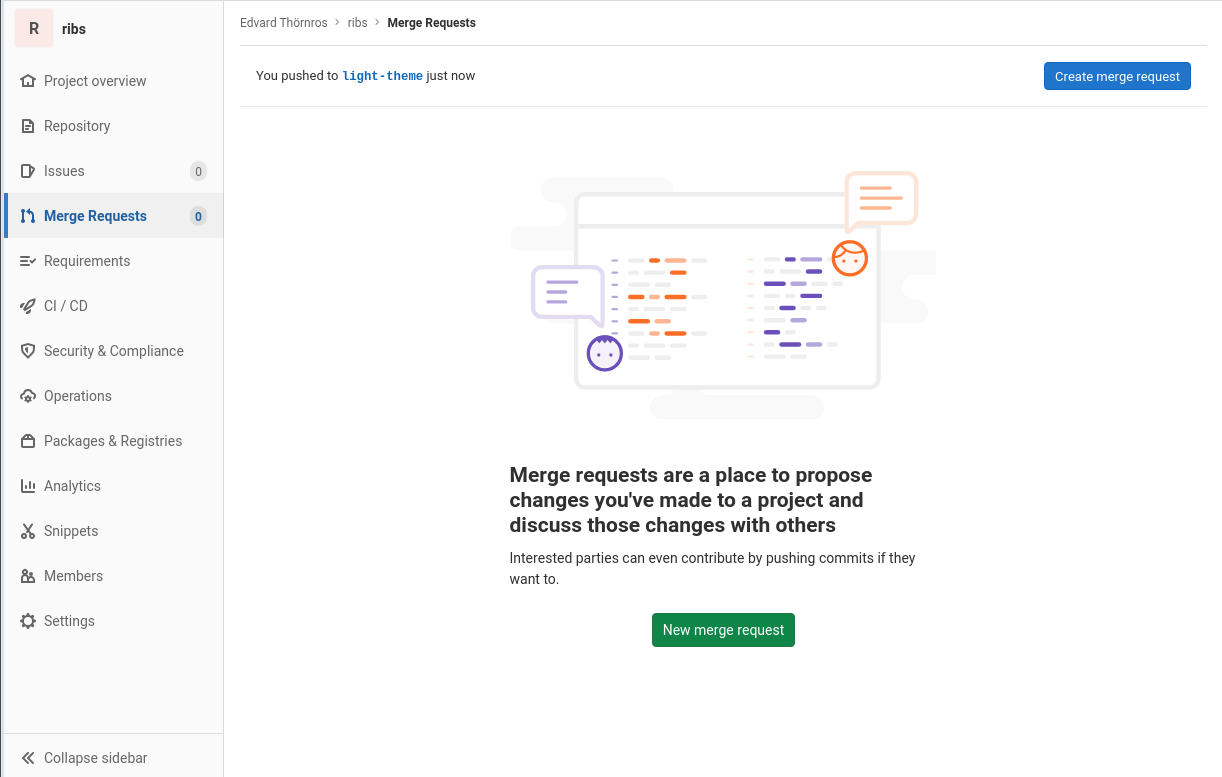
\includegraphics[width=\linewidth]{merge-request/mr-menu-empty.png}
\end{frame}

\begin{frame}[fragile]
  \frametitle{Creating your first Merge Request -- Describe what you've done}
  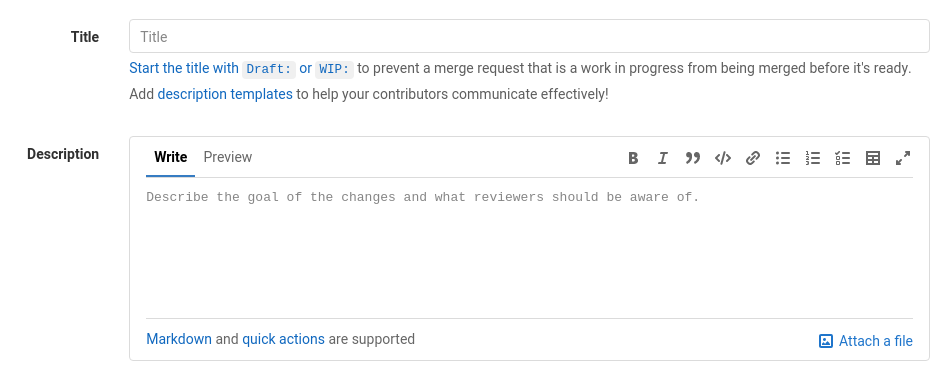
\includegraphics[width=\linewidth]{merge-request/mr-create-01-empty.png}
\end{frame}

\begin{frame}
  \frametitle{Creating your first Merge Request -- How to describe what you've done}
  \begin{itemize}[<+->]
    \item Title
    \begin{itemize}[<+->]
      \item Very short (one sentence)
      \item Explain what the change does
      \item If you can't explain in a short sentence, you should \emph{probably}
            have split it up more. Maybe next time ;)
    \end{itemize}
    \item Description
      \begin{itemize}[<+->]
        \item Long-form
        \item Begin with the \emph{why}
        \item Explain what you've done broadly
      \end{itemize}
  \end{itemize}
\end{frame}

\begin{frame}[fragile]
  \frametitle{Creating your first Merge Request -- Describe what you've done}
  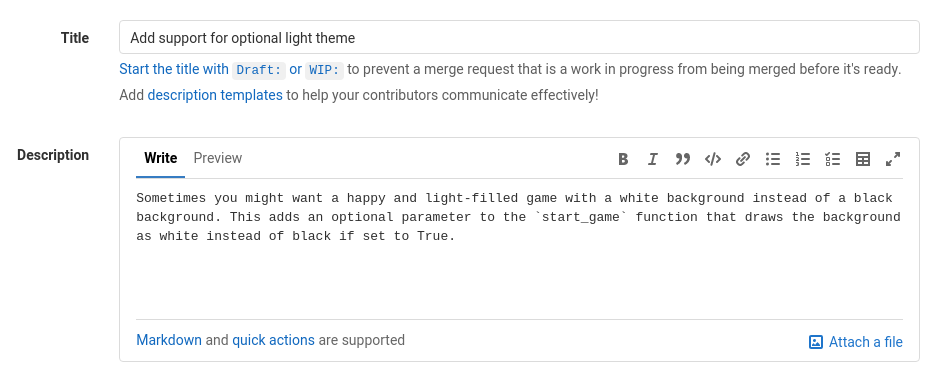
\includegraphics[width=\linewidth]{merge-request/mr-create-01-text.png}
\end{frame}

\begin{frame}[fragile]
  \frametitle{Creating your first Merge Request -- Specify who reviews}
  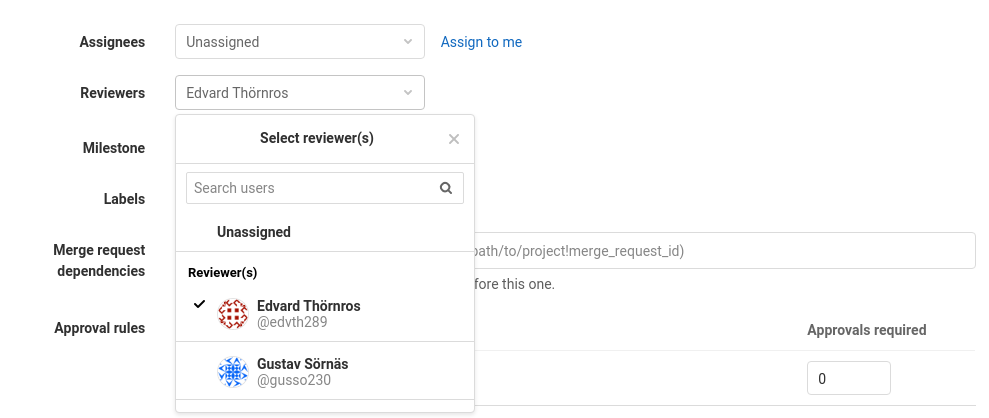
\includegraphics[width=\linewidth]{merge-request/mr-create-03.png} % reviewer
\end{frame}

\begin{frame}
  \frametitle{Creating your first Merge Request -- But who reviews?}
  Who reviews depends on the project and your team.

  \begin{itemize}
    \item Everyone
    \item XX\%
    \item Specific people for specific types of changes
    \item A representative from each sub-team
  \end{itemize}
\end{frame}

\begin{frame}[fragile]
  \frametitle{Creating your first Merge Request -- Send it}
  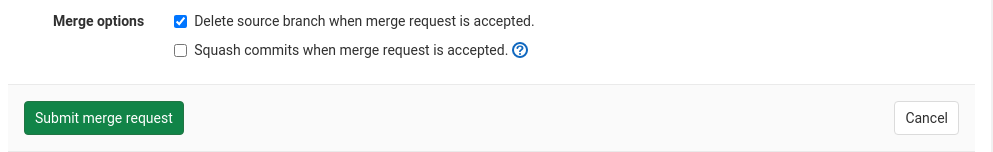
\includegraphics[width=\linewidth]{merge-request/mr-create-04.png} % submit-button
\end{frame}

\begin{frame}[fragile]
  \frametitle{Creating your first Merge Request -- Send it}
  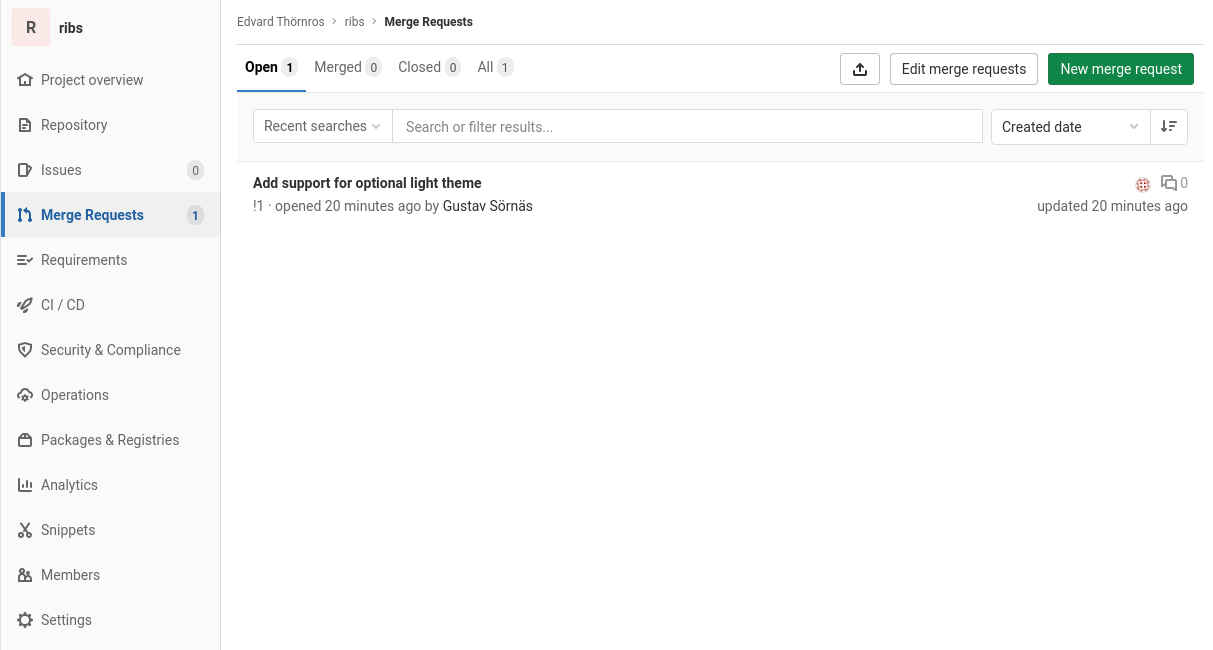
\includegraphics[width=\linewidth]{merge-request/mr-menu-created.png}
\end{frame}

\subsection{Reading your first Merge Request}

\begin{frame}[fragile]
  \frametitle{Reading your first Merge Request}

  Sometimes people want to give you code. That's fun and should be appreciated! \\[1em]
  Here is how you do just that.

\end{frame}

\begin{frame}[fragile]
  \frametitle{Reading your first Merge Request -- The call to action}
  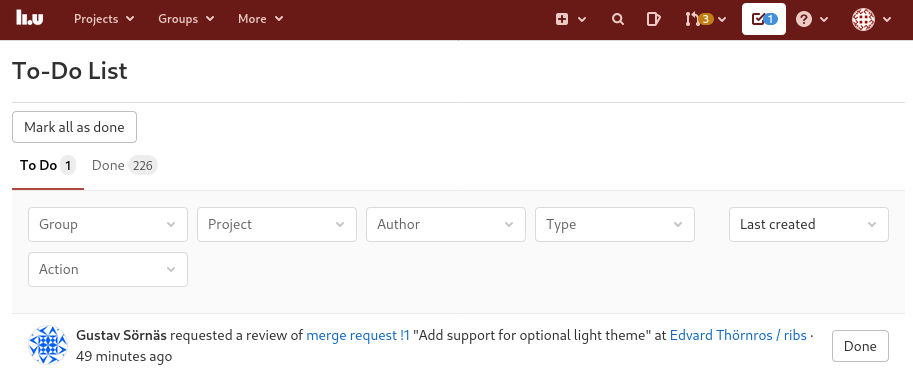
\includegraphics[width=\linewidth]{gitlab-first-review/01-notification.png}
\end{frame}

\begin{frame}[fragile]
  \frametitle{Reading your first Merge Request -- So that's what they did}
  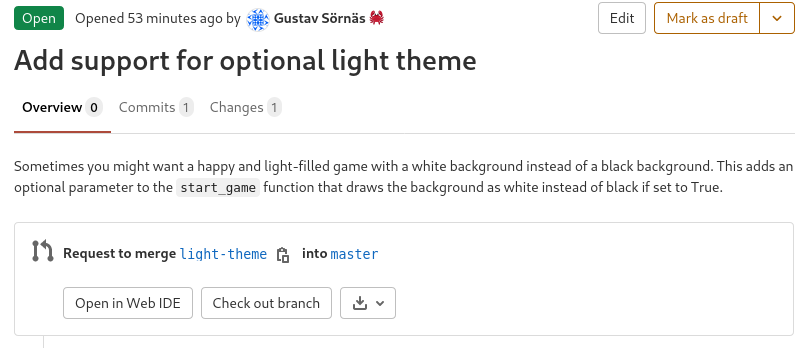
\includegraphics[width=\linewidth]{gitlab-first-review/02-reding.png}
\end{frame}

\begin{frame}[fragile]
  \frametitle{Reading your first Merge Request -- But where to look?}
  
\includegraphics[width=\linewidth]{gitlab-first-review/03-changes.png}
\end{frame}

\begin{frame}[fragile]
  \frametitle{Reading your first Merge Request -- Looking at the diff}
  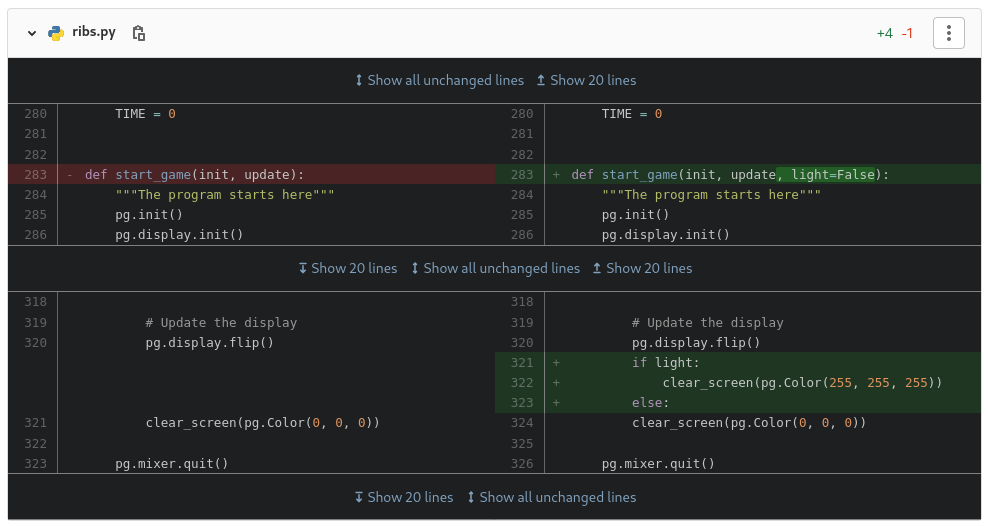
\includegraphics[width=\linewidth]{gitlab-first-review/04-thediff.png}
\end{frame}

\begin{frame}[fragile]
  \frametitle{Reading your first Merge Request -- Spotting a mistake}
  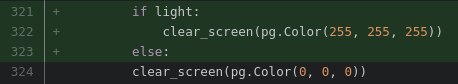
\includegraphics[width=\linewidth]{gitlab-first-review/05-oopsie.png}
\end{frame}

\begin{frame}[fragile]
  \frametitle{Reading your first Merge Request -- Leaving a comment}
  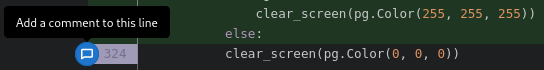
\includegraphics[width=\linewidth]{gitlab-first-review/06-comment.png}
\end{frame}

\begin{frame}[fragile]
  \frametitle{Reading your first Merge Request -- Leaving \emph{constructive} feedback}
  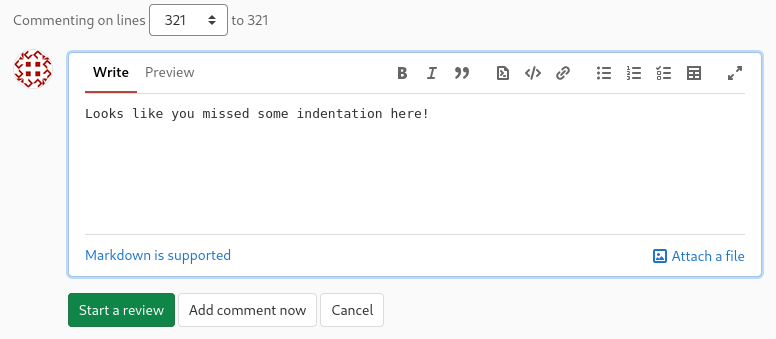
\includegraphics[width=\linewidth]{gitlab-first-review/07-suggestion.png}
\end{frame}

\begin{frame}[fragile]
  \frametitle{Reading your first Merge Request -- Can we do more?}
  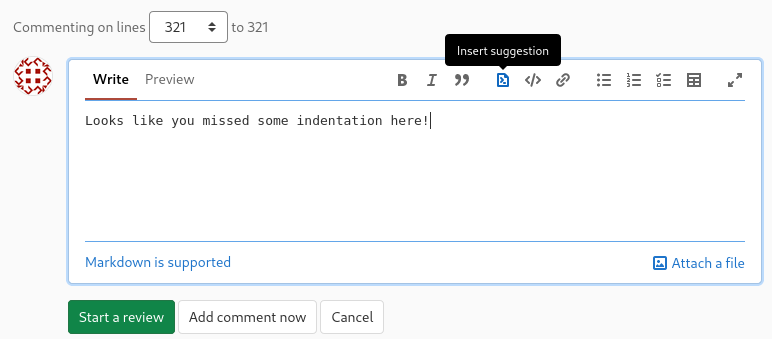
\includegraphics[width=\linewidth]{gitlab-first-review/08-sugg.png}
\end{frame}

\begin{frame}[fragile]
  \frametitle{Reading your first Merge Request -- Being extra helpful}
  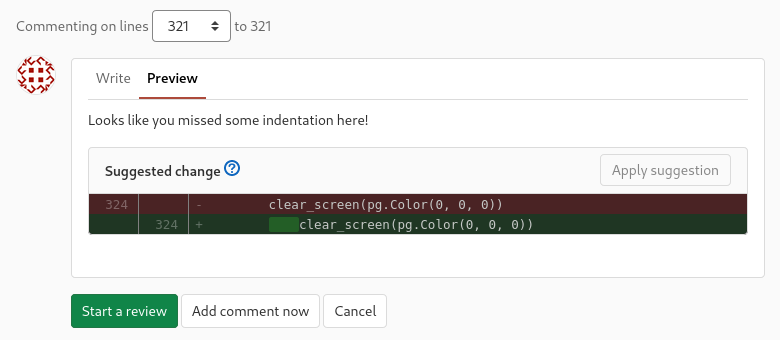
\includegraphics[width=\linewidth]{gitlab-first-review/09-preview.png}
\end{frame}

\begin{frame}[fragile]
  \frametitle{Reading your first Merge Request -- Wrapping it up}
  
\includegraphics[width=\linewidth]{gitlab-first-review/10-submit.png}
\end{frame}

\begin{frame}[fragile]
  \frametitle{Reading your first Merge Request -- Key points}

  Some pointers for being the best reviewer in town
  \begin{itemize}[<+->]
    \item \emph{ALWAYS START BY RUNNING}, don't review stuff that doesn't work
    \item Be constructive and civil
    \item Add suggestions if you know what you want
    \item Ask if stuff is confusing
    \item Propose additions
    \item Don't be afraid to say no -- some code is just bad
    \item Don't take 3 weeks to review
  \end{itemize}
\end{frame}

\subsection{Project management}

\begin{frame}[fragile]
  \frametitle{Project management -- Commit messages}
  \vspace{1em}

  A message describing what has been done.
  \vspace{1em}

  \keyword{Do}
  \begin{itemize}
    \item \dots keep the first line short
    \item \dots maybe add details after the first line
  \end{itemize}
  \vspace{1em}

  \pause

  \keyword{Don't}
  \begin{itemize}
    \item \dots write everything, people can read code
    \item \dots hammer your keyboard
    \item \dots add version numbers
  \end{itemize}
  \vspace{1em}

\end{frame}

\begin{frame}[fragile]
  \frametitle{Project management -- Commit messages example}
  \small
  \begin{verbatim}
Documentation/git-clone.txt: document race with --local

When running 'git clone --local', the operation may
fail if another process is modifying the source
repository. Document that this race condition is
known to hopefully help anyone who may run into it.
  \end{verbatim}
  Taken from git's git-repo.
\end{frame}

\begin{frame}[fragile]
  \frametitle{Project management -- Tags}
  
  A name for a commit. Useful for releases, easy to find.
  \vspace{1em}
  Branches that doesn't move.

\end{frame}

\begin{frame}[fragile]
  \frametitle{Project management -- feature branches}

  \keyword{Idea} \\
  Feature branches! Doing the work on a branch so master always works. \\
  \vspace{1em}

  \keyword{Pros}
  \begin{itemize}[<+->]
    \item Always a working version
    \item Encourages tiny features
    \item Pairs great with issues
    \item You \emph{should} never have broken code
  \end{itemize}
  \vspace{1em}

  Maybe try feature branches! If you want more, you can look at git-flow, taking
  things one step further, but has a little bit more complexity.

\end{frame}

\begin{frame}[fragile]
  \frametitle{Project management -- git $\sim$flow$\sim$ visualized}
  \tikzset{->,        % edges are arrows
           >=stealth  % arrow heads are bold
  }

  \centering
  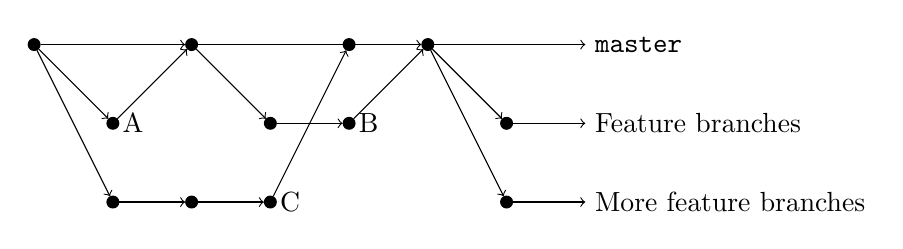
\begin{tikzpicture}[
      dot/.style={circle, draw=black, fill=black, minimum size=1.5mm, inner sep=0pt},
      ]
      \node at (0,0) [dot]  (A) {};
      \node at (1,-1) [dot] (B) {};
      \coordinate [label=right:{A}] (branchA) at (B);
      \draw [->] (A) -- (B);
      \node at (2,0) [dot]  (C) {};
      \draw [->] (B) -- (C);
      \draw [->] (A) -- (C);
      \coordinate [label=right:\texttt{master}] (master) at (7,0);
      \coordinate [label=right:{Feature branches}] (master) at (7,-1);
      \pause{}
      \node at (3,-1) [dot] (D) {};
      \draw [->] (C) -- (D);
      \node at (4,-1) [dot] (E) {};
      \coordinate [label=right:{B}] (branchB) at (E);
      \draw [->] (D) -- (E);
      \node at (5,0) [dot]  (F) {};
      \draw [->] (E) -- (F);
      \draw [->] (C) -- (F);

      \pause{}

      \node at (1,-2) [dot] (H) {};
      \draw [->] (A) -- (H);
      \node at (2,-2) [dot] (I) {};
      \draw [->] (H) -- (I);
      \node at (3,-2) [dot] (J) {};
      \coordinate [label=right:{C}] (branchC) at (J);
      \draw [->] (I) -- (J);
      \node at (4,0) [dot]  (K) {};
      \draw [->] (J) -- (K);
      \coordinate [label=right:{More feature branches}] (master) at (7,-2);
      \pause{}
      \node at (6,-1) [dot] (G) {};
      \draw [->] (F) -- (G);
      \draw [->] (F) -- (7,0);
      \draw [->] (6,-1) -- (7,-1);
      \draw [->] (6,-2) -- (7,-2);

      \node at (6,-2) [dot] (M) {};
      \draw [->] (F) -- (M);
  \end{tikzpicture}
\end{frame}

\begin{frame}[fragile]
  \frametitle{Project management -- CI} % not always needed etc

  \keyword{Idea} \\
  Make a server deploy your code. Run some unit-tests so you don't have to.
  \vspace{1em}

  \keyword{Pros}
  \begin{itemize}[<+->]
    \item No need to run tests
    \item Easier and faster to spot faults
    \item Convenient
  \end{itemize}
  \vspace{1em}

  Might be a bit overkill for a lab, but amazing for projects.

\end{frame}

\begin{frame}[fragile]
  \frametitle{Project management -- CI usecases} % not always needed etc

  Some simple usecases for CI, can easily be set up.
  \vspace{1em}
  \begin{itemize}
    \item Try to compile your project
    \item Run automated tests
    \item Check the formatting of the code
    \item Compile \LaTeX{} to PDFs
  \end{itemize}

\end{frame}

\begin{frame}[fragile]
  \frametitle{Project management -- gitignore}

  \keyword{Idea} \\
  Tell git to ignore files. Lets you be lazy.
  \vspace{1em}

  \keyword{Ignore}
  \begin{itemize}
    \item<2-> Large binary files \textsuperscript{*}
    \item<3-> Temporary files \& log files
    \item<4-> Build output
    \item<5-> Editor files \textsuperscript{**}
  \end{itemize}
  \vspace{1em}

  \visible<6->{More `guidelines' than actual rules.}
  \vspace{1em}

  \visible<2->{\small \textsuperscript{*} Game developers beware \\}
  \visible<5->{\small \textsuperscript{**} Some editors (e.g. VS Code and JetBrains) like to live in git-repos \\}
\end{frame}

\section{Final stretch}
\subsection{Advanced commands}

\begin{frame}[fragile]
  \frametitle{Some more commands (bonus round)}
  These commands can be scary and confusing, and hard to `undo'. Worth a google if you
  want to get more use out of git.
  \vspace{1em}
  
  \command{git worktree} -- Looking at other branches \\
  \command{git cherry-pick} -- Stealing commits \\
  \command{git stash} -- WIP commits \\
    
\end{frame}

\subsection{Finding help}

\begin{frame}[fragile]
  \frametitle{Finding help}

  Human contact \\
  \hspace{1em} LiTHe kod's meetups -- Tuesdays from 17:15 late into the night, \\
  \vspace{1em}
  \pause

  In your terminal at your fingetips \\
  \hspace{1em} \command{man git} -- Exhaustive, good if you know what you want \\
  \hspace{1em} \command{man giteveryday} -- Short description of commands \\
  \hspace{1em} \command{man gittutorial} -- A guide for getting started \\
  \hspace{1em} \command{man git <subcommand>} -- Exhaustive information about a subcommand\\
  \vspace{1em}
  \pause

  From the web, just a GET away \\
  \hspace{1em} \url{git-scm.com/doc} -- Links and reference manual \\
  \hspace{1em} \url{lithekod.se/gitcheatsheet/} -- LiTHe kods cheat-sheet \\
  \hspace{1em} \url{shorturl.at/jpCDQ} -- GitHub's cheat-sheet \\
  \hspace{1em} \url{shorturl.at/tuLO3} -- Flowchart by Justin Hileman for messes\\

\end{frame}

\begin{frame}[fragile]
  \begin{center}
    \Huge Thanks for your time! \\[0.75em]
    \small Brought to you by LiTHe kod
  \end{center}
\end{frame}
\end{document}
